%!TEX root = ../report.tex
\documentclass[report.tex]{subfiles}
\begin{document}
    \chapter{Evaluation and Results}

    \section{Experiment Description}

    % Describe the experiments/evaluation you are performing to analyse your method.
    \paragraph*{Objective}

    % The primary objective of these experiments is to evaluate the efficacy of three multimodal sensor fusion deep neural network models on two diverse public datasets for object detection in a range of adverse weather conditions. This study aims to understand how tightly-coupled, data-driven multimodal sensor fusion can enhance object detection capabilities in environments where traditional methods may falter due to poor visibility and unpredictable weather elements.

    % This study aims to understand how tightly-coupled, data-driven multimodal sensor fusion can enhance object detection capabilities in environments where traditional methods may falter due to poor visibility and unpredictable weather elements.

    % This study aims to 
    % - Understand how tightly-coupled multimodal sensor fusion can enhance object detection capabilities in environments where conventional methods may falter due to poor visibility and unpredictable weather elements.
    % - Highlight the importance of complementary sensors suit for robust object detection in adverse weather conditions.

    % The primary objective of these experiments is to critically evaluate the efficacy of three multimodal sensor fusion deep neural network models on two diverse public datasets, specifically designed for object detection under a range of adverse weather conditions. This study is conducted with a dual aim. Firstly, it seeks to understand how tightly-coupled multimodal sensor fusion can significantly enhance object detection capabilities, particularly in environments where conventional methods may falter. This faltering is often due to poor visibility and the unpredictability of weather elements, which pose substantial challenges to standard detection techniques. Secondly, the study highlights the importance of employing a complementary suite of sensors. This approach is crucial for ensuring robust object detection in adverse weather conditions, suggesting that the integration of diverse sensor modalities can offer a more comprehensive and reliable solution in challenging environmental contexts.

    The primary objective of these experiments is to critically evaluate the efficacy of three multimodal sensor fusion deep neural network models on two diverse public datasets, specifically designed for object detection under a range of adverse weather conditions. Conducted with a dual aim, this study focuses on:

    \begin{itemize}
        \item \textbf{Understanding Tightly-Coupled Multimodal Sensor Fusion}: Investigating how the integration of multiple sensor types can significantly enhance object detection capabilities in environments where traditional methods are less effective. This is particularly relevant in scenarios with poor visibility and unpredictable weather elements, where standard detection techniques may struggle.
        \item \textbf{Highlighting the Importance of Complementary Sensors}: Emphasizing the necessity of employing a suite of complementary sensors for robust object detection in challenging weather conditions. This approach underlines the value of diverse sensor modalities working in concert to provide a more reliable and comprehensive solution for object detection in adverse environmental contexts.
    \end{itemize}

    \paragraph*{Relevance to Adverse Weather Conditions}

    % Adverse weather conditions, such as heavy rain, fog, and snow, pose significant challenges to the accuracy of object detection systems. This research directly addresses these challenges by integrating multimodal sensor data, which is crucial for enhancing the robustness and reliability of object detection in such environments. The approach adopted in this study is anticipated to make a substantial contribution to fields that are critically dependent on weather conditions, like autonomous navigation and outdoor surveillance, by improving operational efficiency and safety in diverse weather scenarios.

    % - Certain commonly used sensors like Camera and Lidar face significant problems in working with inclement weather conditions like heavy rain, fog, and snow. Where as radar proves to be robust to these weather conditions. This research directly addresses these challenges by integrating multimodal sensor data, which is crucial for overall robustness and reliability of object detection in such environments. The approaches adopted in this study is anticipated to make a substantial overview to fields that are critically dependent on weather conditions, like autonomous navigation and outdoor surveillance, by improving operational efficiency and safety in diverse weather scenarios.

    This research tackles the significant challenges posed by adverse weather conditions such as heavy rain, fog, and snow, which greatly affect the accuracy of object detection systems essential in autonomous navigation and outdoor surveillance. Acknowledging the limitations of commonly used sensors like cameras and Lidar in inclement weather, contrasted with the robustness of radar, the study emphasizes integrating multimodal sensor data to bolster the robustness and reliability of object detection in these environments. This study provides a comprehensive overview and detailed analysis of existing top methods, elucidating their efficacy and limitations in diverse weather scenarios, thereby informing best practices in the field.


    


    \section{Experimental Setup}

    Describe your experimental setup in detail.

    %  Include 
    % - dataset split
    % - training settings
    % - hardware used


    % For SAF FCOS
        %  Use this in experiment section
        % - Training Implementation

        %     - It uses SGD with momentum and weight decay, and train for 12 epochs. The official implementation uses batch size of 16 with LR of 0.01 but due to computational limitations, we have used LR 0.001 with reduced batch size 8. It uses warmup scheme for the first few iterations of training.

        %     The training process involves Stochastic Gradient Descent (SGD) with momentum and weight decay, spanning 12 epochs. While the official implementation opts for a batch size of 16 and a learning rate of 0.01, computational constraints led us to use a reduced batch size of 8 and a learning rate of 0.001. A warmup scheme is employed during the initial iterations of training.

        % % TODO: MOVE this section to experiment setup section
        % % \textbf{Dataset split}: 
        % \paragraph*{Dataset Split}
        % The method limits its focus on detecting vehicular obstacles such as — bicycles, cars, motorcycles, buses, trailer, and trucks—collectively categorized as 'vehicles' for simplified classification. Pedestrians are excluded due to radar detection limitations in the nuScenes dataset. Emphasis is placed on front camera data from nuScenes, with the dataset split detailed in Figure \ref{fig:saffcos_data_split}.

        % \begin{figure}[h!]
        %     \centering
        %     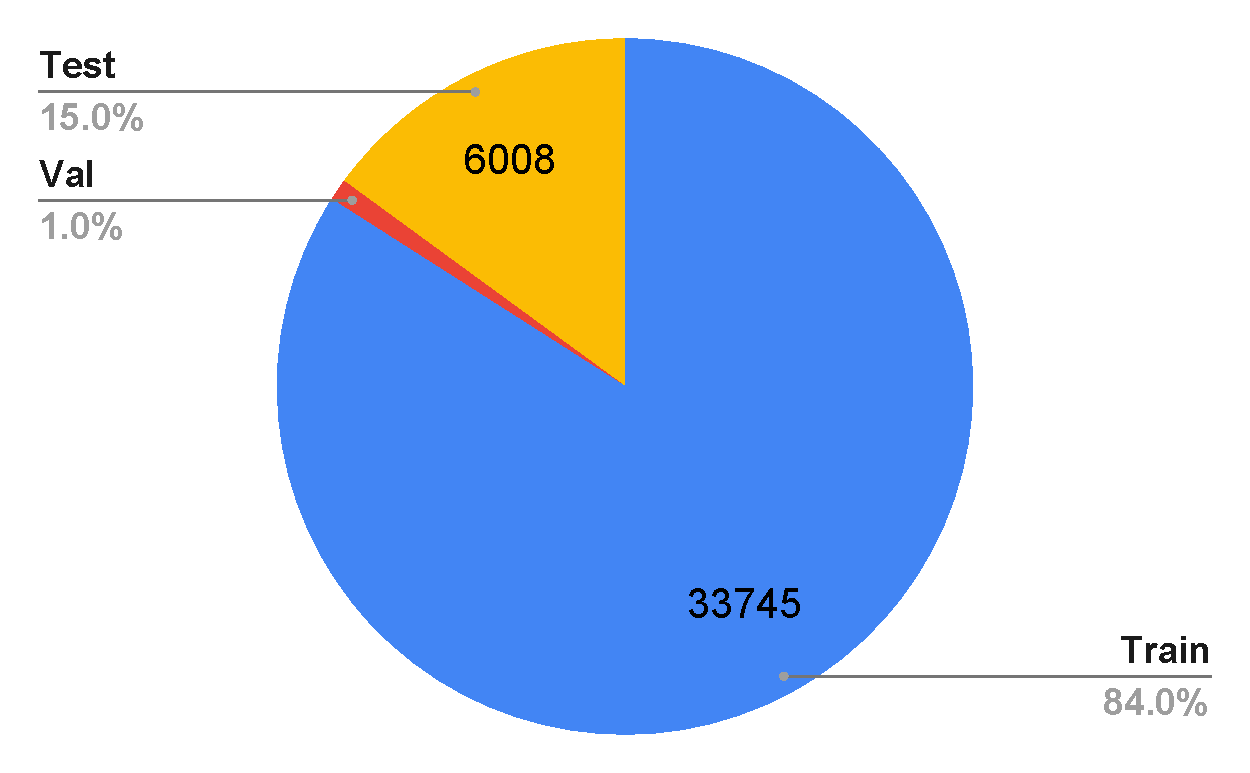
\includegraphics[width=0.5\textwidth]{images/methods/saf_fcos/data_split.pdf}
        %     \caption{Data split of nuScenes dataset. Total samples: 40157. Note: this is a custom dataset split chosen by the authors.}
        %     \label{fig:saffcos_data_split}
        % \end{figure}

    \section{Results}

    Describe the results of your experiments in detail.

\end{document}
